\documentclass{article}
\usepackage[utf8]{inputenc}
\setlength\parindent{0pt}
\usepackage{multirow}
\usepackage{graphicx}
\usepackage{siunitx}
\usepackage{float}
\usepackage{derivative}
\usepackage{amsmath,amssymb}


\title{Assignment 2 description and solutions \\ CTA200H}
\author{Lechung Xing - 1004705170 }
\date{May 8th 2020}

\begin{document}

\maketitle

\section{Question 1}
\subsection{Methods}
In order to plot the complex number z on a 2D plane, I separated z and c(the fixed point $x + iy$) into Real and Imaginary parts corresponding to x and y (axis) components, respectively. I found the expression \(Z_{n+1}= [(ReZ_n)^2-(ImZ_n)^2+x] + 2i[(ReZ_n)(ImZ_n) + y]\) for the sequence \(Z_{n+1} = (Z_n)^2 + c, Z_0 = 0\) as n increases. To test the divergence, I selected some c points with iteration steps varying from $10 to 50$ and computed the \(|z|^2\)for each step. The iteration terminated if \(|z|^2\) is larger than 2, which indicated the sequence is diverging under the initial choice of c. I created a n-dim array to partition the domain of c into a \(Matrix_{n\times{n}}\) so that I can collect the diverging c points and marked them with colours to distinguish from the bounded ones. I attempted to demonstrate the rate of divergence for the diverging c points according to the relative difference between their  \(|z|^2\) value (i.e. the magnitude of the entries in \(Matrix_{n\times{n}} = np.abs(z)\)).
\begin{figure}[H]
    \centering
    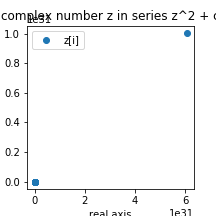
\includegraphics[scale=0.7]{diverge(1,1).png}
    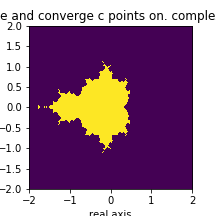
\includegraphics[scale=0.7]{2colours.png}
    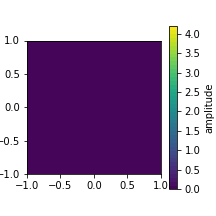
\includegraphics[scale=0.5]{colorbar.png}
    \caption{a) The set of c points confined within a 4 by 4 square are plotted on the complex plane for $c = 1 + 1i$. b) The shaded region represents the c points that generate diverging sequence \(z_{i+1}=(z_i)^2 + c\). The yellow region shows the c points that yield bounded sequences. c)The rate of divergence with color bar generated from n-dim matrix entries. The color resembles the $3rd$ axis apart from x and y axis. }
    \label{fig:Q1}
\end{figure}

\section{Discussion}
In Fig. 1a, since $c = 1 + 1i$ yields diverging sequence from the $8th$ iteration step, the blue dots are far away from each other as expected. In Fig. 1b, the bounded c points are bounded by an open ball of radius 2 centered at the origin. The n-dim array of \(|z|^2\) contains different entries, unlike the homogeneous color as shown in Fig. 1c.


\section{Question 2}
\subsection{Methods}
I implemented the initial condition: $N = 1000, S(t) + I(t) + R(t) = N for any t\in[0, 200]$ to solve the ODE by using the $Scipy.odeint$ package. The parameters: $\beta and \gamma$ determine the slope of the first derivative of S, I, R. I expect S to decrease while I increases in the beginning followed by the delayed increase in R. To take into account of the death rate arising from the infected population, I added $D(t)*I(t)$ to $dI/dt$ and subtracted the death term from $dR/dt$ to satisfy the initial condition. 

\begin{figure}[H]
    \centering
    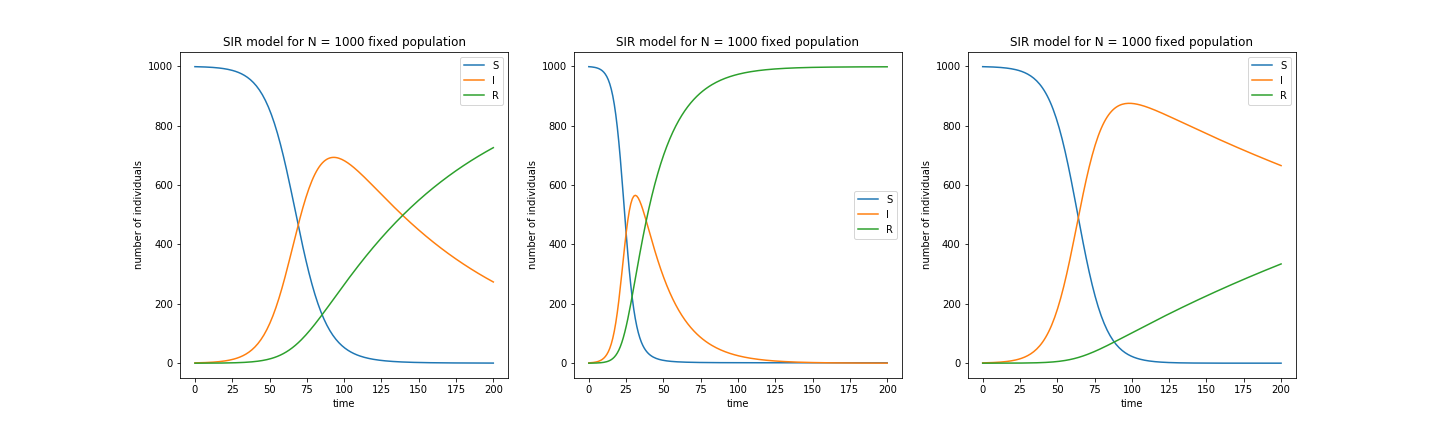
\includegraphics[scale=0.31]{3curvesSIR.png}
    \includegraphics[scale=0.8]{4curvesSIR (1).png}
    \caption{a) The S(t), I(t), R(t) curves plotted for \(t=200days\), representing the number of vulnerable(not yet affected) individuals, infected individuals and recovered individuals, respectively. The first graph has parameters \(\beta=9\times10^6, \gamma=0.01\), second one with \(\beta=3\times10^6, \gamma=0.05\) and the last one with \(\beta=9\times10^6, \gamma=0.003\). The initial condition is \(S(0)=999, I(0)=1 and R(0)=0\) b)Same as a) with a death term included \(\beta=3\times10^6, \gamma=0.005, death2 = 0.01\). }
    \label{fig:Q2}
\end{figure}

\section{Discussion}
Among the 3 figures in Fig. 2a, the one the middle best represents the disease spreading model with a reasonable infected curve and a flattened out recovered curve. Unlike the first and the third plot, the decaying tails of $I(t)$ and $R(t)$ expanded beyond the 200 days time interval which is too slow for most common diseases. In Fig. 2b, the death rate exceeds the recovered rate near $t = 180days$. Vulnerable but not infected individuals vanished after $t=75days$, they become either recovered or dead as shown in this new model. 


\end{document}